\section{Konzept Druckluft}
\begin{figure}[h!]
	\centering
	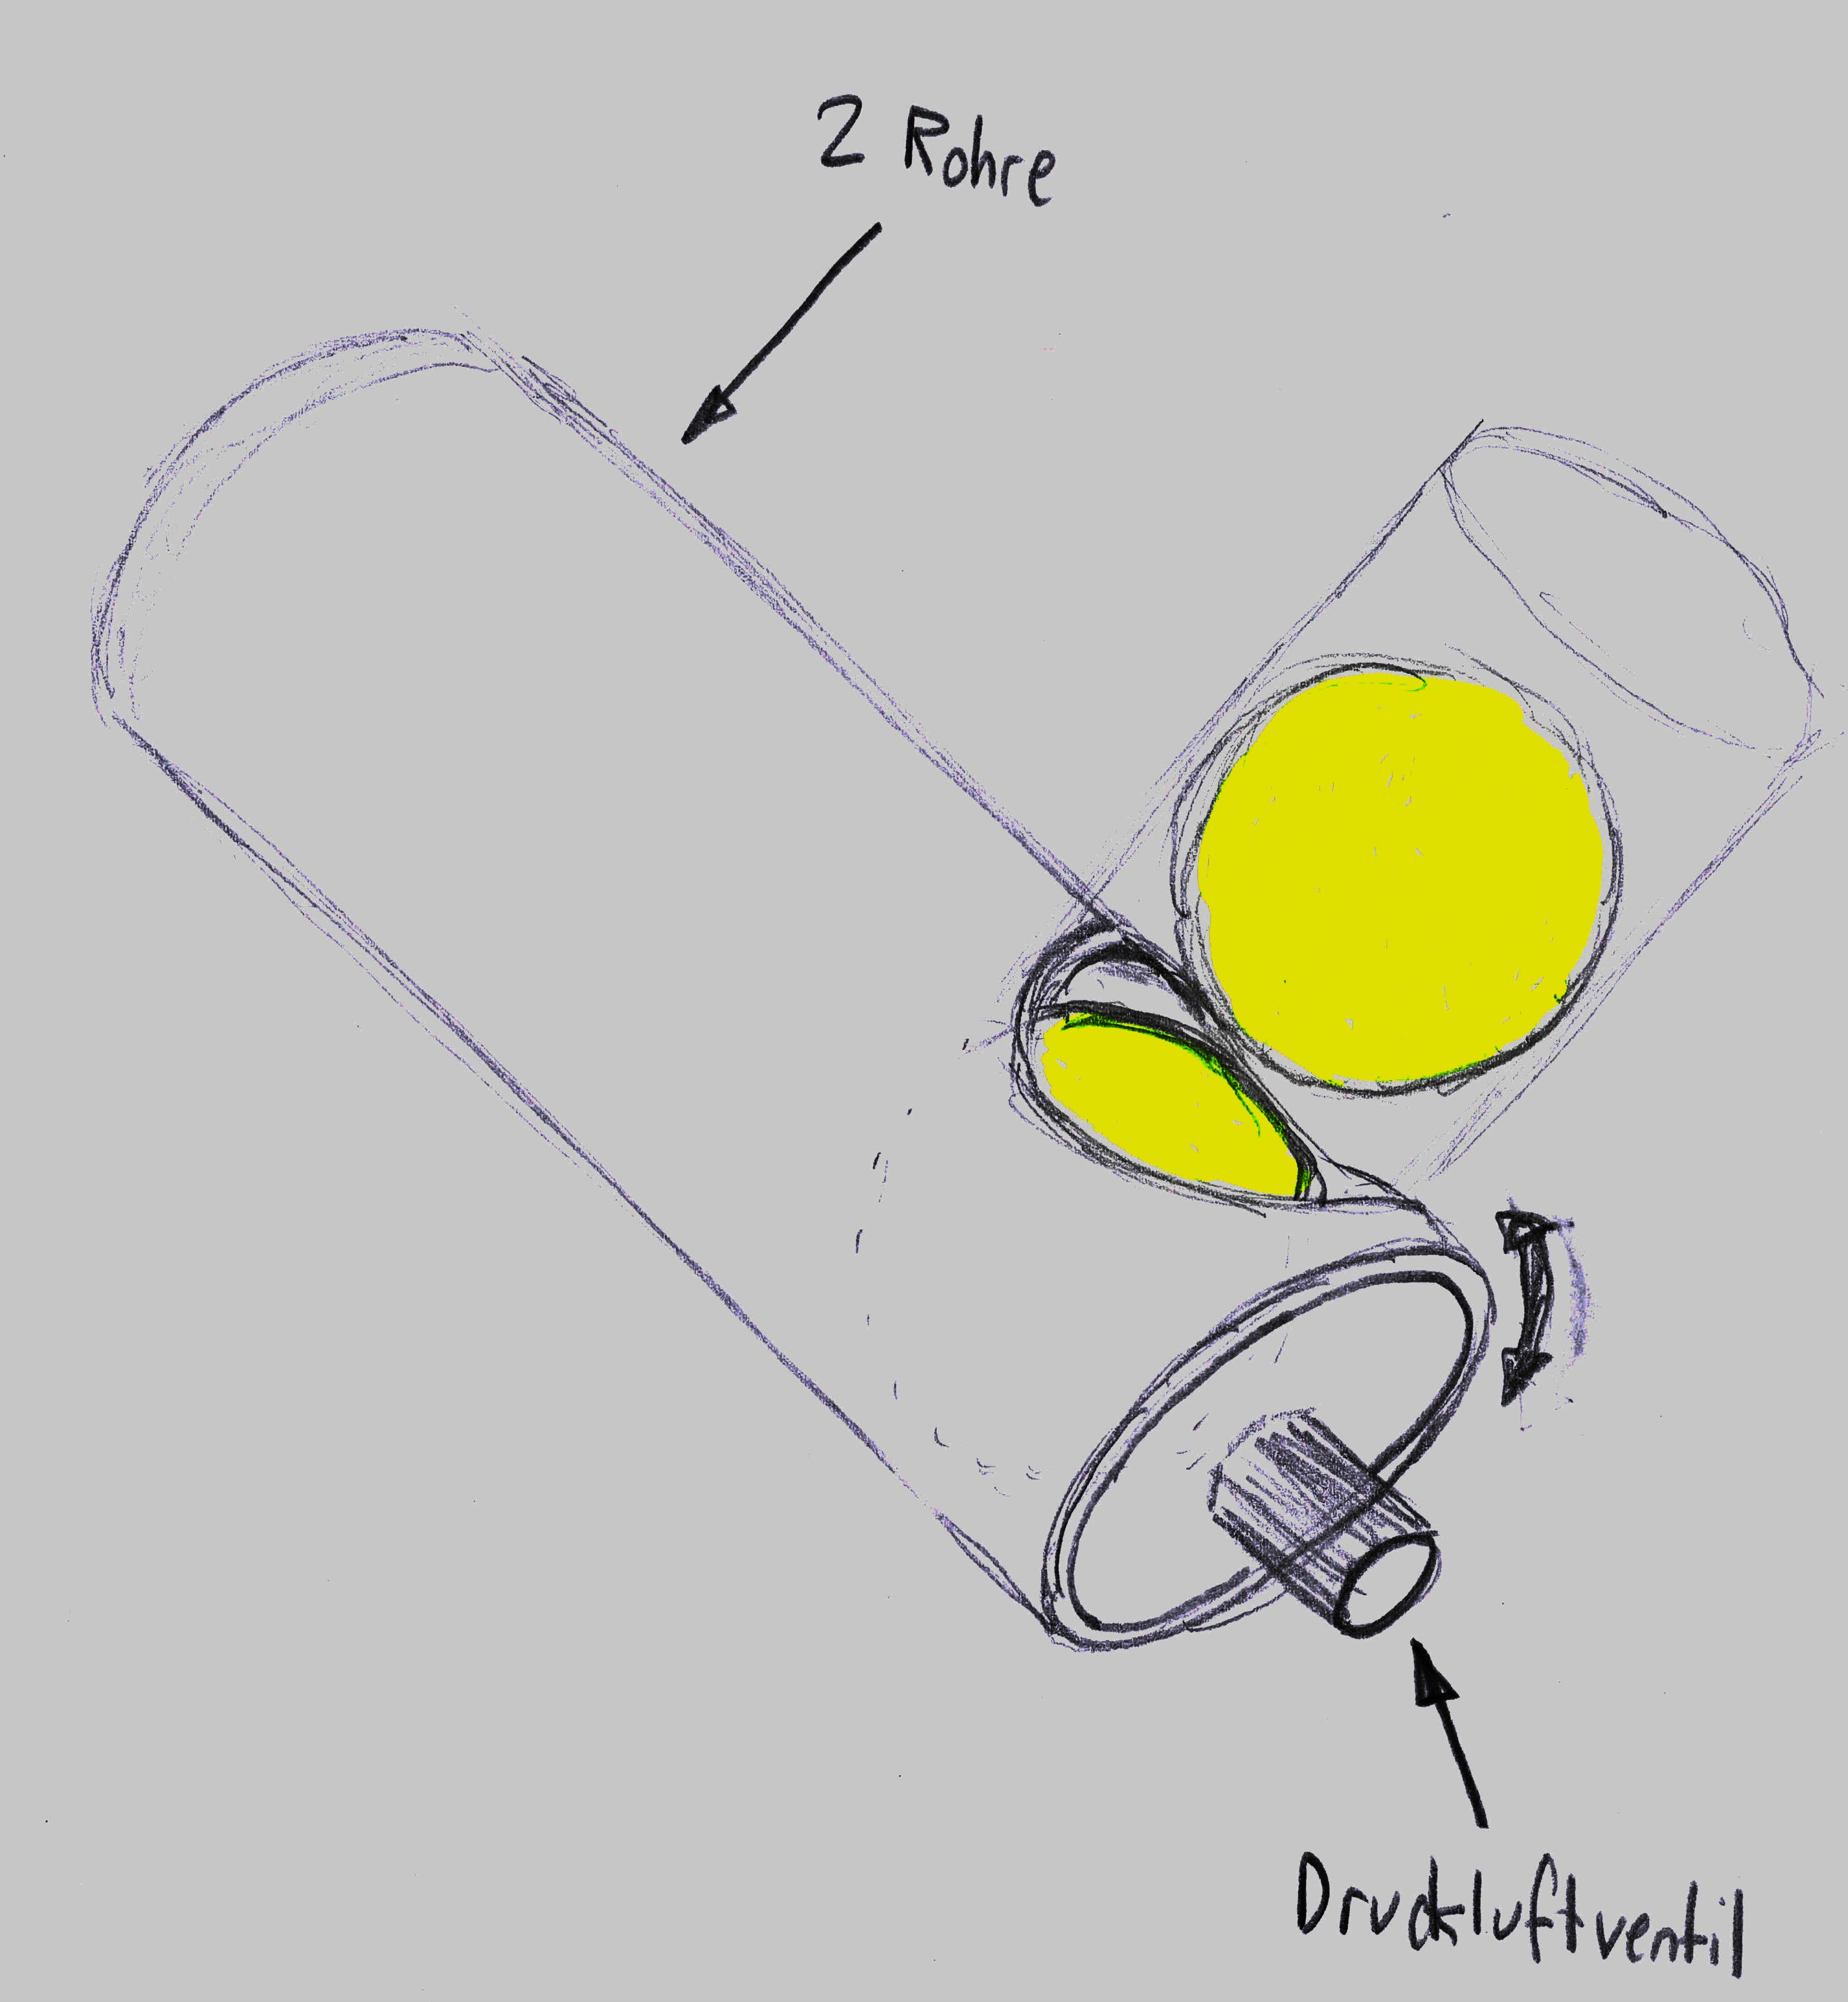
\includegraphics[width=0.4\textwidth]{../../fig/Druckluftrohr.jpg}
	\caption{Druckluftrohr}
	\label{fig:druckluftrohr}
\end{figure}

\subsection{Idee}
Die Idee ist Druckluft zu benutzen, um ein Ball aufs mal durch ein Rohr zu beschleunigen. Es wird der zur Verfügung stehende Druckluftanschluss benutzt. Da die Bälle eine Differenz im Durchmesser bis zu 1 cm haben können, kann das Rohr nicht dicht sein. Aus diesem Grund werden wir ein Rohr benutzen dessen Durchmesser nur wenig grösser ist, als der grösste Ball. Wir werden das Rohr so modifizieren, dass es gerade nach der Aufladezone enger ist, so dass sich alle Bälle dort blockieren. Dank dieser Verengung blockiert sich der Ball und der Luftdruck hinter dem Ball wird grösser, bis genug Druck vorhanden ist um den Ball durch die Verengung zu drücken. Dieser Prozess wird dem Ball genügend Energie geben um bis zum Korb zu fliegen.
Die Nachladung der Bälle kann mit einem zweiten Rohr gemacht werden, der sich um das erste Rohr dreht. Diese Rohre sind beide so geschnitten, dass wenn beide Öffnungen übereinstimmen ein neuer Ball ins erste Rohr fällt. Wenn die beide Schnitte nicht übereinstimmen ist das erste Rohr dicht.

\subsection{Annahmen}
Um sicherzustellen dass das Konzept funktioniert, muss die Schrumpfung und der Ball eng anliegend, so dass die Druckluft genügend Druck aufbauen kann, um den Ball abzuschiessen. Deswegen darf der Durchmesser der Bälle nicht zu unterschiedlich sein. 

\subsection{Vor- und Nachteile}
Falls der Durchmesser der Bälle zu unterschiedlich ist, kann es bei einigen Bällen passieren, dass sie nicht den Korb treffen, weil der Druck nicht genügend oder zu gross war. Weil das Rohr etwas grösser ist als die Bälle, gibt es die Möglichkeit, dass die Bälle beim Wurf links oder rechts weg fliegen oder sogar einklemmen. Der Vorteil dieses Konzept sind die Kosten. Da hier kein Motor für die Beschleunigung genutzt wird, werden die Kosten von dieses Teil ausfallen und auch die nötige Batterie für die Schrittmotoren kann deutlich kleiner sein.
